\begin{technical}
{\Large\textbf{Swapped Axes and Emergent Behavior: A Minimal Model of the Creeper}}\\[0.1em]

Entity models in early Minecraft were defined using bounding boxes in Java. 
Each model was specified via constructor calls like:
\[
\begin{aligned}
\texttt{ModelBox(}&\texttt{name, x, y, z,} \\
&\texttt{length, height, width)}.
\end{aligned}
\]
For passive mobs, proportions typically followed:
\begin{align*}
\texttt{length} &> \texttt{height}, \\
\texttt{length} &\approx 1.2, \\
\texttt{height} &\approx 0.9.
\end{align*}

Due to a developer error, \texttt{length} and \texttt{height} were swapped:
\[
(\ell,\ h,\ w)\ \mapsto\ (h,\ \ell,\ w).
\]
This produced a tall, narrow model. Define the pig’s geometry as:
\[
G_{\text{pig}} = [0,\ell] \times [0,h] \times [0,w],
\]
and the resulting Creeper geometry as:
\[
G_{\text{creeper}} = [0,h] \times [0,\ell] \times [0,w].
\]
With \( \ell \approx 2.0 \), \( h \approx 1.0 \), the resulting model appeared upright and columnar.


\vspace{0.3em}
\noindent\textbf{Visual Mutation and Face Topology}\\[0.5em]
The model was assigned Minecraft’s leaf texture. A simple face overlay was defined
on the front-facing surface using pixel coordinates:
\begin{align*}
\texttt{eyes} &:\quad (x,y) \in \{(3,12), (10,12)\}, \\
\texttt{mouth} &:\quad (x,y) \in \{(5,6), (4,4), (10,4)\}.
\end{align*}

\vspace{0.3em}
\noindent\textbf{AI Composition and Swell Behavior}\\[0.5em]
The Creeper’s actions derive from prioritized AI goals:
\begin{align*}
&\texttt{Goal 1: LookAtPlayer} \quad (\text{range } R = 6), \\
&\texttt{Goal 2: ApproachPlayer} \quad (\text{speed } v = 0.2), \\
&\texttt{Goal 3: StartSwell} \quad (\text{trigger } r < r_s), \\
&\texttt{Goal 4: Explode} \quad (\text{delay } \tau = 1.5\,\text{s}).
\end{align*}
Explosion occurs if the player remains within range \( r_s = 2.5 \) blocks for the full
fuse duration. Let \( r(t) \) denote distance to the player at time \( t \). Then:
\[
\texttt{if } r(t) < r_s \ \forall t \in [t_0, t_0 + \tau], \texttt{Explode()}.
\]
Damage output is modeled by radial falloff:
\[
D(x) = \max\left(0, E_{\max}\left(1 - \frac{\|x - x_0\|}{R}\right)\right),
\]
where \( x_0 \) is the explosion center and \( R \approx 7 \) blocks in air.

\vspace{0.3em}
\noindent\textbf{Reconstruction in TikZ}\\[0.5em]
The diagram below illustrates the result of axis misassignment during model construction.
On the left, the intended pig model appears with a horizontal body and frontal facial features.
On the right, the same parameters are rendered with the \texttt{length} and \texttt{height}
values swapped. This inversion laid the foundation for the Creeper’s distinctive form.

\begin{center}
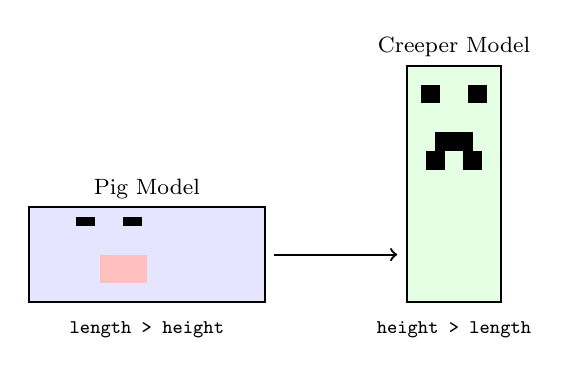
\begin{tikzpicture}[scale=1.2]

% Pig (Horizontal)
\draw[thick, fill=blue!10] (0,0) rectangle (2.5,1);
\node at (1.25,1.2) {\footnotesize Pig Model};

% Eyes
\fill[black] (0.5,0.8) rectangle (0.7,0.9);
\fill[black] (1.0,0.8) rectangle (1.2,0.9);
% Snout
\fill[pink] (0.75,0.2) rectangle (1.25,0.5);

% Creeper (Vertical)
\draw[thick, fill=green!10] (4,0) rectangle (5,2.5);
\node at (4.5,2.7) {\footnotesize Creeper Model};

% Eyes
\fill[black] (4.15,2.1) rectangle (4.35,2.3);
\fill[black] (4.65,2.1) rectangle (4.85,2.3);
% Mouth
\fill[black] (4.3,1.6) rectangle (4.7,1.8);
\fill[black] (4.2,1.4) rectangle (4.4,1.6);
\fill[black] (4.6,1.4) rectangle (4.8,1.6);

% Arrows
\draw[->, thick] (2.6,0.5) -- (3.9,0.5);

% Labels
\node at (1.25,-0.3) {\scriptsize \texttt{length > height}};
\node at (4.5,-0.3) {\scriptsize \texttt{height > length}};

\end{tikzpicture}
\end{center}


\vspace{0.5em}
\noindent\textbf{References:}\\
Persson, M. (2009). \textit{Initial Geometry and Entity Source}. Mojang.\\
Minecraft Wiki. (2025). \textit{Entity Models and AI Mechanics}. \texttt{https://minecraft.wiki}
\end{technical}
